\documentclass[../ala_hataile.tex]{subfiles}
\begin{document}
\clearpage

\includepdf[pages=12-13, pagecommand={}]{sisasivut_19062018.pdf}
\raggedbottom
\twocolumn[\section{Geotieteiden opiskelu}]
\subsection*{Mitä on geotieteet?}
\begin{figure}[b!]
	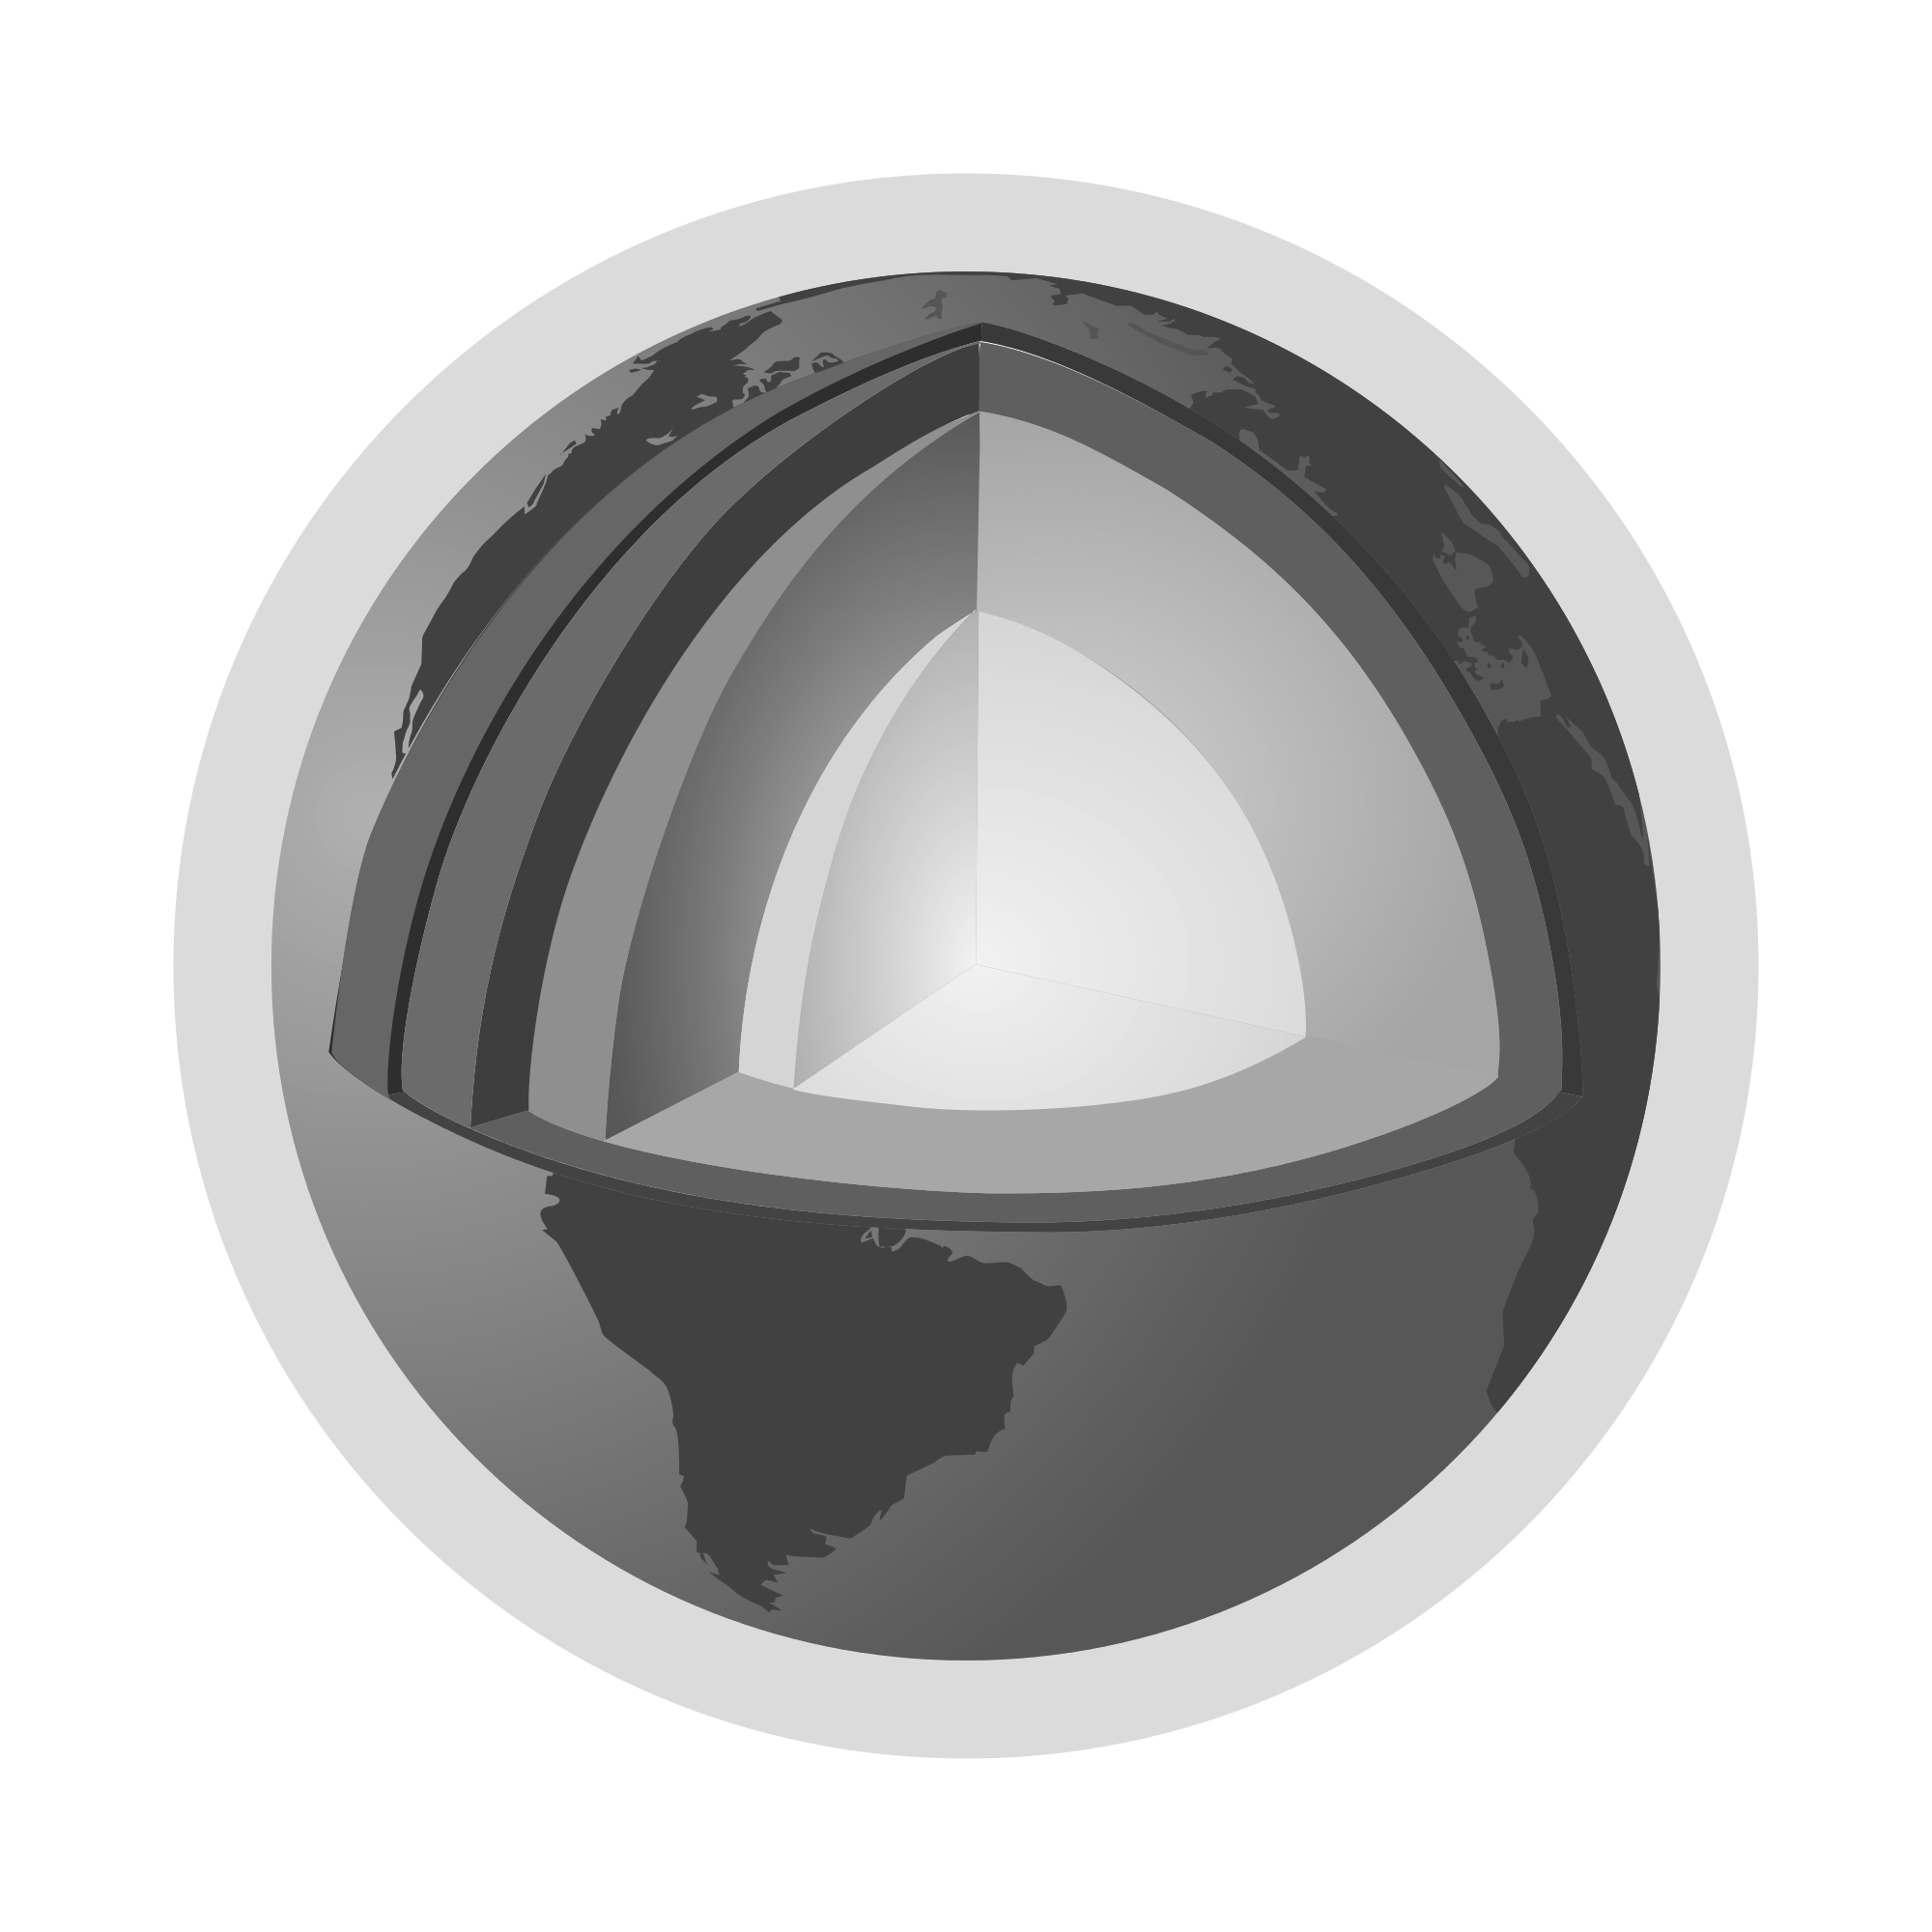
\includegraphics[width=\columnwidth]{maapallohalki.png}
\end{figure}
Geotieteiden piiristä löytyy neljä tieteen\-alaa: geologia, paleontologia, geofysiikka ja geokemia. Geotieteiden opiskelijana saat aivan uudenlaisen näkökulman ympäröivään luontoon: näkemämme luonto on geologisten prosessien muodostamaa ja muokkaamaa. Kenttäopetus on geotieteiden opetuksen kivijalka.

Perus- ja aineopinnoissa opit perusasiat maapallon prosesseista, koostumuksesta, rakenteesta ja historiasta, opit tunnistamaan mineraaleja, kivilajeja, maalajeja sekä fossiileja ja ymmärtämään niiden merkityksen. Muut tieteenalat kuten kemia, fysiikka, matematiikka ja tilastotiede antavat tarvittavan taustatuen geotieteiden opinnoille. Luentosalien lisäksi opintoja toteutetaan monenlaisissa ympäristöissä, kuten opetuslaboratorioissa, kenttäkursseilla tutkimusasemilla tai opintomatkoilla muille mantereille. Opinnot sisältävät luentojen lisäksi runsaasti itsenäistä ja ryhmätyöskentelyä, erilaisia harjoituksia sekä työelämään valmentavaa sisältöä.

Geotieteiden opiskelijat muodostavat tiiviin ja aktiivisesti toimivan yhteisön, jonka keskiössä ovat geologian opiskelijajärjestö Vasara~ry ja geofysiikan opiskelijajärjestö Geysir.

\subsection*{Kasvihuone}
Vasaran opiskelijatila, Kasvis eli Kasvihuone, sekä sen vieressä sijaitseva Appro\-sali tulevat fukseille nopeasti tutuksi. Perimätiedon mukaan huoneen nimi tulee kirjoitus\-virheestä pohja\-piirustuksessa, johon huone oli merkattu kahvi\-huoneen sijaan kasvi\-huoneeksi. Kasvikselta löytyy mm.\,jääkaappi, mikro ja teenkeitin, minkä lisäksi Vasaralla on oma kahvi\-myynti. Kasviksella jokainen siivoaa omat jälkensä ja tapoihin kuuluu käyttää omaa kuppia. Tietokone on kaikkien käytettävissä ja siltä löytyy myös Vasaran digitaalinen tenttiarkisto. Kasviksen koneen tausta\-kuvan vaihtaminen on vasaralaisen pieniä ja halpoja huveja.

\subsection*{Liikuntaa}
Vasaralla on joka torstai klo~14--16 liikuntavuoro Kumpulan UniSportilla. Liikunta\-vuoro on vasaralaisille maksuton, eikä siis edellytä UniSportin asiakkuutta. Vuorolla harrastettavista lajeista päätetään yhdessä Vasaran sportti\-saitti-ryhmässä Facebookissa. Lisätietoa saa Vasaran liikunta\-vastaavilta.

Geysir ja Vasara pelaavat vuosittain perinteisen vappu\-pesiksen Vallilan kentällä. Tulethan täydentämään joukkueita ensi vappuna!
\begin{figure}[b!]
	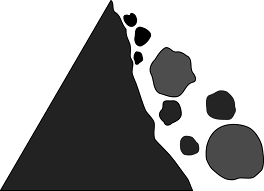
\includegraphics[width=\columnwidth]{kivivyory.png}
\end{figure}

\subsection*{Digiloikka}
Koska maasto-opetus on kallista ja mahdollinen maasto-opetus\-kausi Suomen sää\-olo\-suhteissa lyhyt ja arvaamaton, pilotoi geotieteiden kandi\-ohjelma syksystä 2018 alkaen virtuaalista maasto-opetusta. Opetus perustuu GigaPan-panoraama\-kuviin sekä virtuaalisiin ekskursio\-materiaaleihin. Seuraa digi\-loikan etenemistä blogissa! \url{https://blogs.helsinki.fi/geotieteidendigiloikka/}
\subsection*{Kysymyksiä?}
Mikäli haluat tietää lisää geotieteistä, apua tarjoavat kandiohjelman ja maisteriohjelman opiskelija\-edustajat Theo Männistö, Sonja Silvennoinen, Ville Nenonen ja Lotta Ylä-Mella, Geysirin ja Vasaran hallitukset, sekä HOPS-ohjaajat Aku Heinonen (petrologia ja kallioperägeologia), Anu Kaakinen (sedimentologia ja stratigrafia), Emilia Koivisto (sovellettu geo\-fysiikka) ja Seija Kultti (ympäristö\-geologia ja paleo\-klimatologia).

Mia Kotilainen on geotieteiden kandiohjelman koulutussuunnittelija. Hänen kauttaan voi kysyä kaikista tieteenalaan sekä kursseihin liittyvistä asioista ja pyytää hyväksymismerkinnät geotieteiden kokonaisuuksista.

\twocolumn[\section{Geotieteiden kursseja}]
Geotieteiden kurssit järjestetään Physicumissa ja Exactumissa. Mikro\-skooppi\-harjoitukset pidetään Approsalin vieressä olevassa luokassa. Sen vierestä löytyy tietokoneluokka, jonka koneille on asennettu 3D-mallinnukseen ja paikkatiedon käsittelyyn tarvittavia ohjelmistoja.
\subsection*{Perusopinnot}
\begin{figure}[!b]
	\centering
	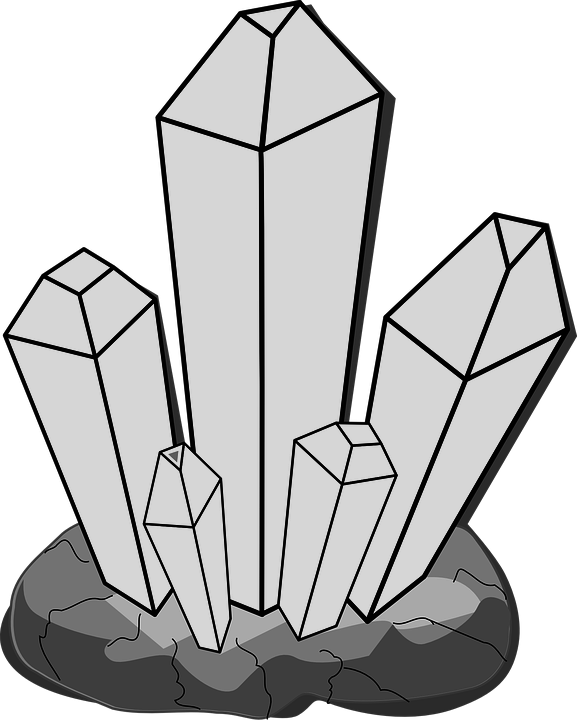
\includegraphics[width=\columnwidth]{crystal-307264_960_720.png}
\end{figure}
\subsubsection*{Geologiset prosessit (5~op)}
Miten laattatektoniikka toimii ja miksi maanjäristyksiä on siellä missä niitä on? Miten vuoristot muodostuvat ja miten oma kallioperämme on muodostunut? Mitä kauniisti poimuttunut juoni on joutunut käymään läpi? Mitä meteoriitit saavat aikaan iskeytyessään Maan pinnalle? Mitä meteoriitit oikeastaan edes ovat? Jos nämä kysymykset askarruttavat, tämä kurssi on sinua varten! 

Kurssi nivoo yhteen kaikki suurimmat maapalloon vaikuttavat prosessit. Nopeasti käväistään myös pallomme ulkopuolella. Täällä opit muun muassa Maan rakenteen ja fysikaaliset ominaisuudet sekä Maata muokkaavat endogeeniset ja eksogeeniset prosessit. Koska asiaa on paljon, tahti on melko nopea. Lisäksi luvassa on mukava (lue: haastava) määrä Mastering Geologyn tarjoamia tehtäviä. Onneksi aihe sentään on mielenkiintoinen!

\subsubsection*{Maan ja elämän kehitys (5~op)}
Mitä tarkoittaa geologinen aikakäsitys? Miten mantereet olivat sijoittuneena dinosaurusten aikaan? Millaisia otuksia Maan historiassa on elellyt ja kuinka elämä on kehittynyt? Tuliko ordoviki\-kausi ennen siluuria vai toisin päin? Mikä edes on ordoviki tai siluuri?

Maapallon ja elämän tarina on tarinoista suurin. Kurssi kertoo tämän tarinan yleispiirteet ja selittää sen tieteellisen taustan, keskeiset prosessit ja vuorovaikutukset kivikehän, ilmakehän ja elokehän välillä. Kurssia opettaa suuri määrä eri aloihin erikoistuneita luennoitsijoita ja professoreja, joten jokaiselle varmasti löytyy se mieluisin aihe ja mielenkiintoisin professori. 
   
\subsubsection*{Geologiset materiaalit (5~op)}
Kivetkin kiinnostaa? No, geologeja ainakin! Maapallo ja muut planeetat koostuvat geologisista materiaaleista: mineraaleista, kivilajeista ja sedimenteistä. Kurssilla opetetaan niiden tunnistamisen ja luokittelun perusteet luonnonnäytteissä. 

Kivilajit ja sedimentit koostuvat mineraaleista ja mineraalit ovat kiteisiä aineita. Kurssi alkaakin kiteiden symmetrian ja kiderakenteen tarkastelulla. Se on pohja mineraalien ominaisuuksien ymmärtämiselle. Eri mineraaleilla on erilaiset fysikaaliset ja kemialliset ominaisuudet, joita kurssin toisessa osiossa käytetään mineraalien tunnistamiseen suoraan käsinäytteistä. Myöhempien harjoitusten tarkoituksena on oppia tunnistamaan yleisimpiä mineraaleja sekä kivi- ja maalajeja. 
\begin{figure}[b!]
	\centering
	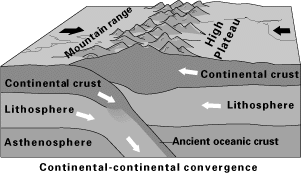
\includegraphics[width=\columnwidth]{Continental-continental_convergence_Fig21contcont.png}
\end{figure}

Kurssi on jaettu kolmeen osaan teemoittain: kiteet ja mineraalit, maalajit ja viimeisenä kivilajit, ja kurssi pitää sisällään sekä tuhdin määrän teoriaa että käytännön harjoituksia kiteiden, mineraalien ja kivilajien tunnistamiseen. Pidä varasi, sillä tämän kurssin jälkeen et voi olla tutkiskelematta lenkkipolulta löytämiäsi kivenmurikoita!
\subsubsection*{Luonnonvarat ja ympäristö (5~op)}
Luonnonvarojen esiintyminen, jakautuminen ja kestävä käyttö? Globaalit geologiset riskit ja yhteiskunnan kannalta merkittävimmät ympäristögeologiset kysymykset? Jos nämä kuulostavat mielestäsi mielenkiintoisilta, tulet pitämään tästä kurssista. Kurssilla perehdytään eri luonnonvaroihin, mm.\,metalleihin ja fossiilisiin polttoaineisiin, sekä niiden yhteiskunnallisiin ja globaaleihin vaikutuksiin. Lisäksi tärkeitä teemoja ovat ympäristö ja pilaantuminen. 

Kurssiin kuuluu kenttä\-päivä, jossa käydään Viikin jäte\-veden\-puhdistamolla ja Ämmäs\-suon kaato\-paikalla. Erittäin kiinnostavia kohteita sinänsä, mutta pieni vinkki: ei välttämättä kannata mennä kyseiselle retkelle krapulassa\dots
\subsubsection*{Suomen geologinen kehitys (5~op)}
Tiedätkö miltä Suomi näytti kymmenen tuhatta vuotta sitten? Entä pari miljardia vuotta sitten? Kurssilla perehdytään Suomen maa- ja kallioperän tyypillisiin piirteisiin, kehitykseen sekä niihin vaikuttaneisiin tapahtumasarjoihin. Tutuiksi tulevat Runkauksen basaltti, Viipurin batoliitti, Muhoksen hiekka\-kivi ja oikeastaan jokainen iso tai pieni geologinen yksikkö Suomen alueella sekä myöskin jääkauden kulutus-, kuljetus- ja kasaustyöt. 

Kuten moniin muihinkin kursseihin, tähänkin kuuluu kenttäpäivä jos toinenkin, joiden aikana kierretään pää\-kaupunki\-seudulla tutkimassa mm.\,Pihlajamäen hiidenkirnua, Jako\-mäessä muinais\-rantaa ja suota ja Vuo\-saaressa jää\-kauden jälkiä. Ulkoilu, eväiden syönti ja luennoitsijoiden kanssa läpän heittäminen on näillä retkillä parasta!

\subsection*{Aineopintotasoiset kurssit}
\subsubsection*{Hydrogeologia (5~op)}
Jos haluat tietää kaiken ja vähän enemmänkin pohjavedestä, on tämä kurssi tarkoitettu juuri sinulle! Luennoilla pääset piirtelemään nuolia, tarkkailemaan veden valumista eri maalajien läpi, käsittelemään pohjavesiputkia sekä pohtimaan, onko elohopea myrkyllistä, tai että onko bensa-asema pohja\-vesi\-alueen vieressä riski veden\-otolle. Innovatiiviset Mastering Geology "-harjoitukset opettavat sinulle, miten Yhdys\-valloissa käsitellään jätteitä. Varaudu siihen, että vain yksi neljästä videosta aukeaa ongelmitta. 

Kurssin lopussa järjestetään kenttä\-päivä jäte\-veden\-puhdistamolle Säkylään katsomaan, mihin länsi\-suomalainen lika\-vesi valuu. Pieni vinkki tähänkin: jos kurssin aikana tehtävistä tai tentistä tulee kysyttävää, kaikki kysymykset kannattaa ehdottomasti kysyä tunnilla, koska Moodlessa tai sähkö\-postissa kysyessä saa helposti joutua odottelemaan\dots

\subsubsection*{Petrologian teoria (5~op)}
Haluatko nukkua aamuisin pitkään? Ikävä juttu. Juuri kun luulit tietäväsi jotain geologiasta, tällä kurssilla Streck\-eisenin kolmiot iskevät takaisin. Luentojen ohessa käydään läpi mm.\,koko termodynamiikka, kerrotaan mistä kivi syntyy (kivivanhemmat rakastuu ja saa vahinkolapsen), ja nähdään mikä on fluorin ja veden vaikutus termodynaamiseen systeemiin. Taustalle tarvitset oikeastaan vain geotieteiden perusopinnot ja rutkasti kahvia -- petrologian jatkokurssilla tarvitaan sitten oikeasti teddyä.

Kurssilla on valinnainen kolmen päivän ekskursio Kaakkois-Suomen geologisille kohteille. Kurssi on yksi kallio\-perä\-geologian kenttäkurssin pakollisista edeltävistä opinnoista.

\subsubsection*{Introduction to Quantitative Geology (5~op)}
Tällä kolmannen vuoden kurssilla mallinnetaan geotieteiden yhtälöitä Pythonilla. Aaltoyhtälö, diffuusioyhtälö ja muut matemaattiset hirviöt käydään luentojen aikana ensin läpi käsiä heilutellen ja animaatioiden avulla, minkä jälkeen niitä kokeillaan käytännössä lähes valmiilla Python-skripteillä. Kurssin ohessa opit myös englantia ja kuulet hauskoja anekdootteja elävästä elämästä. Tietokoneen käyttötaito on syytä hankkia jo ennen kurssin alkua (ks.\,esim.\,kurssi~FYS1013), sillä kurssin oppimiskäyrä on eksponentiaalisesti jyrkkenevä. Kurssin lopussa sinun pitäisi viimeistään ymmärtää, mikä derivaatta on.

\end{document}